\documentclass[11pt,a4paper]{article}
\usepackage[margin=2.5cm]{geometry}
\usepackage{amsmath,amssymb}
\usepackage{graphicx}
\usepackage{booktabs}
\usepackage{array}
\usepackage{xcolor}
\usepackage{caption}
\usepackage{enumitem}
\usepackage{float}
\usepackage{hyperref}
\hypersetup{colorlinks=true,linkcolor=blue!70!black,citecolor=green!50!black,urlcolor=blue!70!black}
\graphicspath{{figures/}}
\newcommand{\uboone}{MicroBooNE}
\newcommand{\GeVc}{\,\text{GeV}\!/c}
\newcolumntype{L}[1]{>{\raggedright\arraybackslash}p{#1}}
\newcolumntype{C}[1]{>{\centering\arraybackslash}p{#1}}

\begin{document}

\begin{titlepage}
\centering
\vspace*{2cm}
{\LARGE\bfseries Control Regions with Beam-On Data\par}
\vspace{0.5cm}
{\large Measurement of $\nu_\mu + \bar{\nu}_\mu$ Charged-Current Single Pion
Production on Argon in the NuMI Beam\par}
\vspace{0.8cm}
{\large First results with real data; the signal region remains blind\par}
\vspace{0.5cm}
{\normalsize 2026-09-09\par}
\vspace{1.5cm}
{\large Ishanee Pophale, Jarek Nowak\par}
\vspace{0.5cm}
{\normalsize\textit{Lancaster University}\par}
\vspace{2cm}

\begin{abstract}
The four inclusive control regions of the $\mathrm{CC}\,1\mu1\pi Xp$ NuMI analysis have
been opened on beam-on data. This note reports what was processed, the yields and
distributions in each region, and the statistics of the frozen comparison procedure
applied to the data. The signal region has \emph{not} been opened: the beam-on files were
processed into a signal-region-stripped skim, verified to contain no event passing the
signal selection.

Two things must be settled before any of these numbers is read as a statement about the
background model. First, \textbf{no Run-2 beam-on file exists}, so Run~2 is excluded from
the data \emph{and} from the prediction throughout; the comparison covers $85.7\%$ of the
FHC and $76.6\%$ of the RHC exposure. Second, and more seriously, the run-by-run
comparison is not uniform: \textbf{FHC Run~1 sits at a data/prediction ratio of
$0.64$--$0.72$ in the high-statistics regions while every other run period of either beam
mode lies between $1.08$ and $1.25$}. Flux and detector uncertainties are common to the
run periods of a mode and cancel in that comparison, so the difference is not a
systematic of the prediction. The natural explanation is the exposure assumed for the
staged FHC Run-1 beam-on file, which no quantity in this comparison verifies. Until that
is resolved the mode-level ratios of \S\ref{sec:yields} should not be interpreted.

With FHC Run~1 set aside, the remaining five run periods sit coherently $10$--$25\%$ above
the prediction in all four regions. That is a common normalisation offset, the one
direction the frozen global test is explicitly insensitive to, and it is within the
$20$--$30\%$ prediction uncertainty. It is nonetheless coherent across regions of very
different composition, and is the second thing to understand.
\end{abstract}
\end{titlepage}

\tableofcontents
\clearpage

% =============================================================================
\section{What was opened, and what was not}
\label{sec:scope}
% =============================================================================

The analysis is blind in the signal region. Beam-on data were processed with the
control-region skim: an event is written only if it \emph{fails} the complete
signal-region selection \emph{and} satisfies at least one of the four approved
control-region definitions. The written file carries a marker that the cross-section
extraction refuses, and the sideband tools accept a beam-on file only if it carries that
marker. Each processing job re-read its own output and deleted it unless the marker was
present, no written event carried the signal-region flag, and every written event fell in
at least one control region. All eight files passed.

Because the skim keeps every control-region event and discards only events that are in the
signal region or in no region at all, the control-region distributions below are complete:
nothing that belongs in a control region has been dropped.

\begin{table}[H]
  \centering
  \caption{Beam-on files processed. ``Input events'' is the number of entries in the
    PeLEE ntuple; the run range is read from the file and is what fixes the horn-mode
    assignment of the Run-4 sub-periods, which the file names do not always carry. The
    beam-off files of the same production have the mode in their names and the same run
    ranges, which is how 4a/4b are identified as RHC and 4c/4d as FHC.}
  \label{tab:files}
  \small
  \begin{tabular}{lllr}
    \toprule
    Period & File & Run range & Input events \\
    \midrule
    FHC Run 1  & \texttt{run1\_beamon\_beamgood}        & 4952--6748   & 610\,496 \\
    FHC Run 4c & \texttt{beam\_on\_run4c}               & 21286--22269 & 392\,148 \\
    FHC Run 4d & \texttt{beam\_on\_run4d\_fhc}          & 22270--23259 & 228\,821 \\
    FHC Run 5  & \texttt{beam\_on\_run5}                & 24376--25759 & 748\,669 \\
    \midrule
    RHC Run 1  & \texttt{run1\_RHC\_beamon\_beamgood}   & 6748--6998   & 167\,923 \\
    RHC Run 3  & \texttt{run3b\_beamon\_beamgood}       & 14117--17566 & 1\,104\,349 \\
    RHC Run 4a & \texttt{beam\_on\_run4a}               & 19660--19752 & 43\,027 \\
    RHC Run 4b & \texttt{beam\_on\_run4b}               & 19753--21285 & 835\,573 \\
    \bottomrule
  \end{tabular}
\end{table}

\paragraph{The CRT-era trigger flag.} The Run-4 and Run-5 beam-on files carry a
software-trigger flag that is identically zero and no companion pre-CRT flag, exactly the
pattern of the CRT-era beam-off samples. The branch is bound only when the companion
branch is present, so these files keep the fail-open default and are not rejected. Had
that not been the case, Runs~4 and~5 would have processed to zero events silently. This
was verified on the beam-on files directly before processing.

\paragraph{No Run-2 beam-on data.}
The staged files cover run numbers 4952--6998, 14117--17566 and 19660--25759. Nothing
lies in the range 6999--14116, which contains all of Run~2. The exposure the prediction is
normalised to assigns Run~2 $1.268\times10^{20}$~POT in FHC and $2.591\times10^{20}$ in
RHC, so the missing period is $14.3\%$ of the FHC, $23.4\%$ of the RHC and $19.4\%$ of the
combined exposure. Run~2 is therefore dropped from the data and from the prediction ---
the Monte Carlo, the beam-off and the dirt --- everywhere in this note. The beam-off side
of the analysis stands Run~1 in for Run~2 permanently, because beam-off is a
cosmic-only sample matched by run period; that substitution is not available for beam-on
data, which is the measurement.

\begin{table}[H]
  \centering
  \caption{Exposure entering this comparison, against the full exposure the analysis is
    normalised to.}
  \label{tab:exposure}
  \small
  \begin{tabular}{lccc}
    \toprule
    & Runs used & POT used ($10^{20}$) & Fraction of the mode \\
    \midrule
    FHC & 1, 4, 5 & 7.589 & $85.7\%$ \\
    RHC & 1, 3, 4 & 8.491 & $76.6\%$ \\
    \bottomrule
  \end{tabular}
\end{table}

% =============================================================================
\section{Yields and distributions}
\label{sec:yields}
% =============================================================================

The prediction is the same stack as the blind studies: neutrino Monte Carlo scaled per run
to that run's data exposure with the central-value weight, plus the per-run beam-off
sample scaled by its gate ratio, plus the dirt overlay. Unlike the pseudo-data studies,
\emph{nothing is added to the data}: real beam-on data already contains cosmics and dirt,
which here belong to the prediction alone.

\begin{table}[H]
  \centering
  \caption{Control-region yields with beam-on data, summed over the run periods used.
    The prediction components are the neutrino signal contamination, the neutrino
    background, the beam-off and the dirt. \textbf{The mode-level ratios in the last
    column mix the FHC Run-1 anomaly of \S\ref{sec:perrun} with the rest and should not
    be read on their own.}}
  \label{tab:yields}
  \small
  \begin{tabular}{llrrrrrr}
    \toprule
    Mode & Region & Data & Prediction & signal & $\nu$ bkg & beam-off & dirt \\
    \midrule
    FHC & CC$0\pi$    & 10\,660 & 11\,571.0 & 962.3 & 9\,442.8 & 1\,118.1 & 47.8 \\
        & multi-$\pi$ &     109 &     109.6 &  24.3 &     79.6 &      5.7 &  0.1 \\
        & $\pi^0$     &  6\,291 &  6\,327.3 & 562.2 & 5\,119.5 &    635.4 & 10.1 \\
        & cosmic      &      92 &     108.3 &   5.0 &     59.5 &     42.0 &  1.9 \\
    \midrule
    RHC & CC$0\pi$    & 12\,047 & 10\,558.9 & 915.2 & 8\,763.9 &    846.7 & 33.1 \\
        & multi-$\pi$ &     136 &     125.0 &  27.1 &     94.3 &      3.6 &  0.1 \\
        & $\pi^0$     &  8\,092 &  6\,639.5 & 594.0 & 5\,578.8 &    459.7 &  7.0 \\
        & cosmic      &     120 &      89.5 &   5.0 &     58.0 &     25.2 &  1.3 \\
    \bottomrule
  \end{tabular}
\end{table}

\begin{figure}[H]
  \centering
  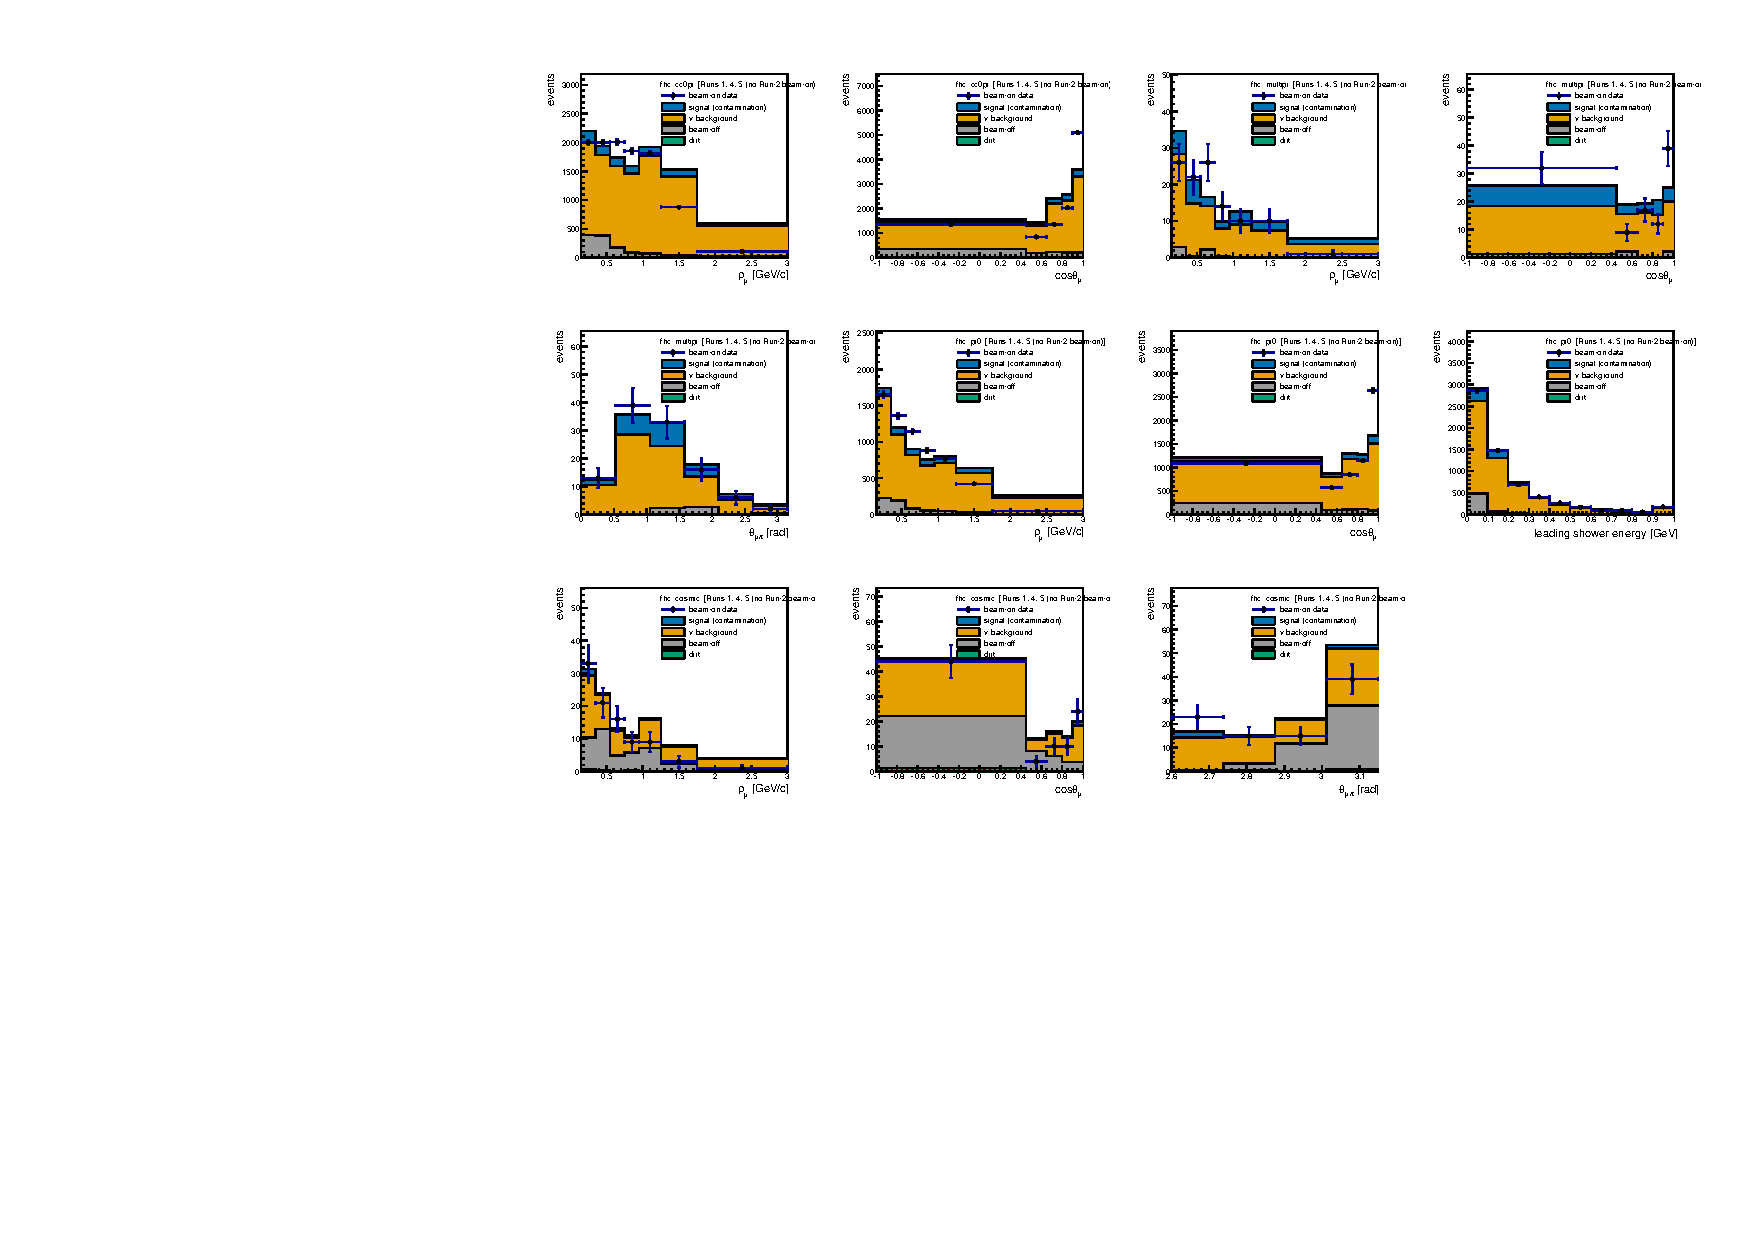
\includegraphics[width=\textwidth]{sideband_data_fhc}
  \caption{FHC control regions with beam-on data (Runs 1, 4, 5). Rows are the CC$0\pi$,
    multi-$\pi$, $\pi^0$ and cosmic regions; the distributions are the frozen ones. Points
    are beam-on data with Poisson errors; the stack is the prediction.}
  \label{fig:data_fhc}
\end{figure}

\begin{figure}[H]
  \centering
  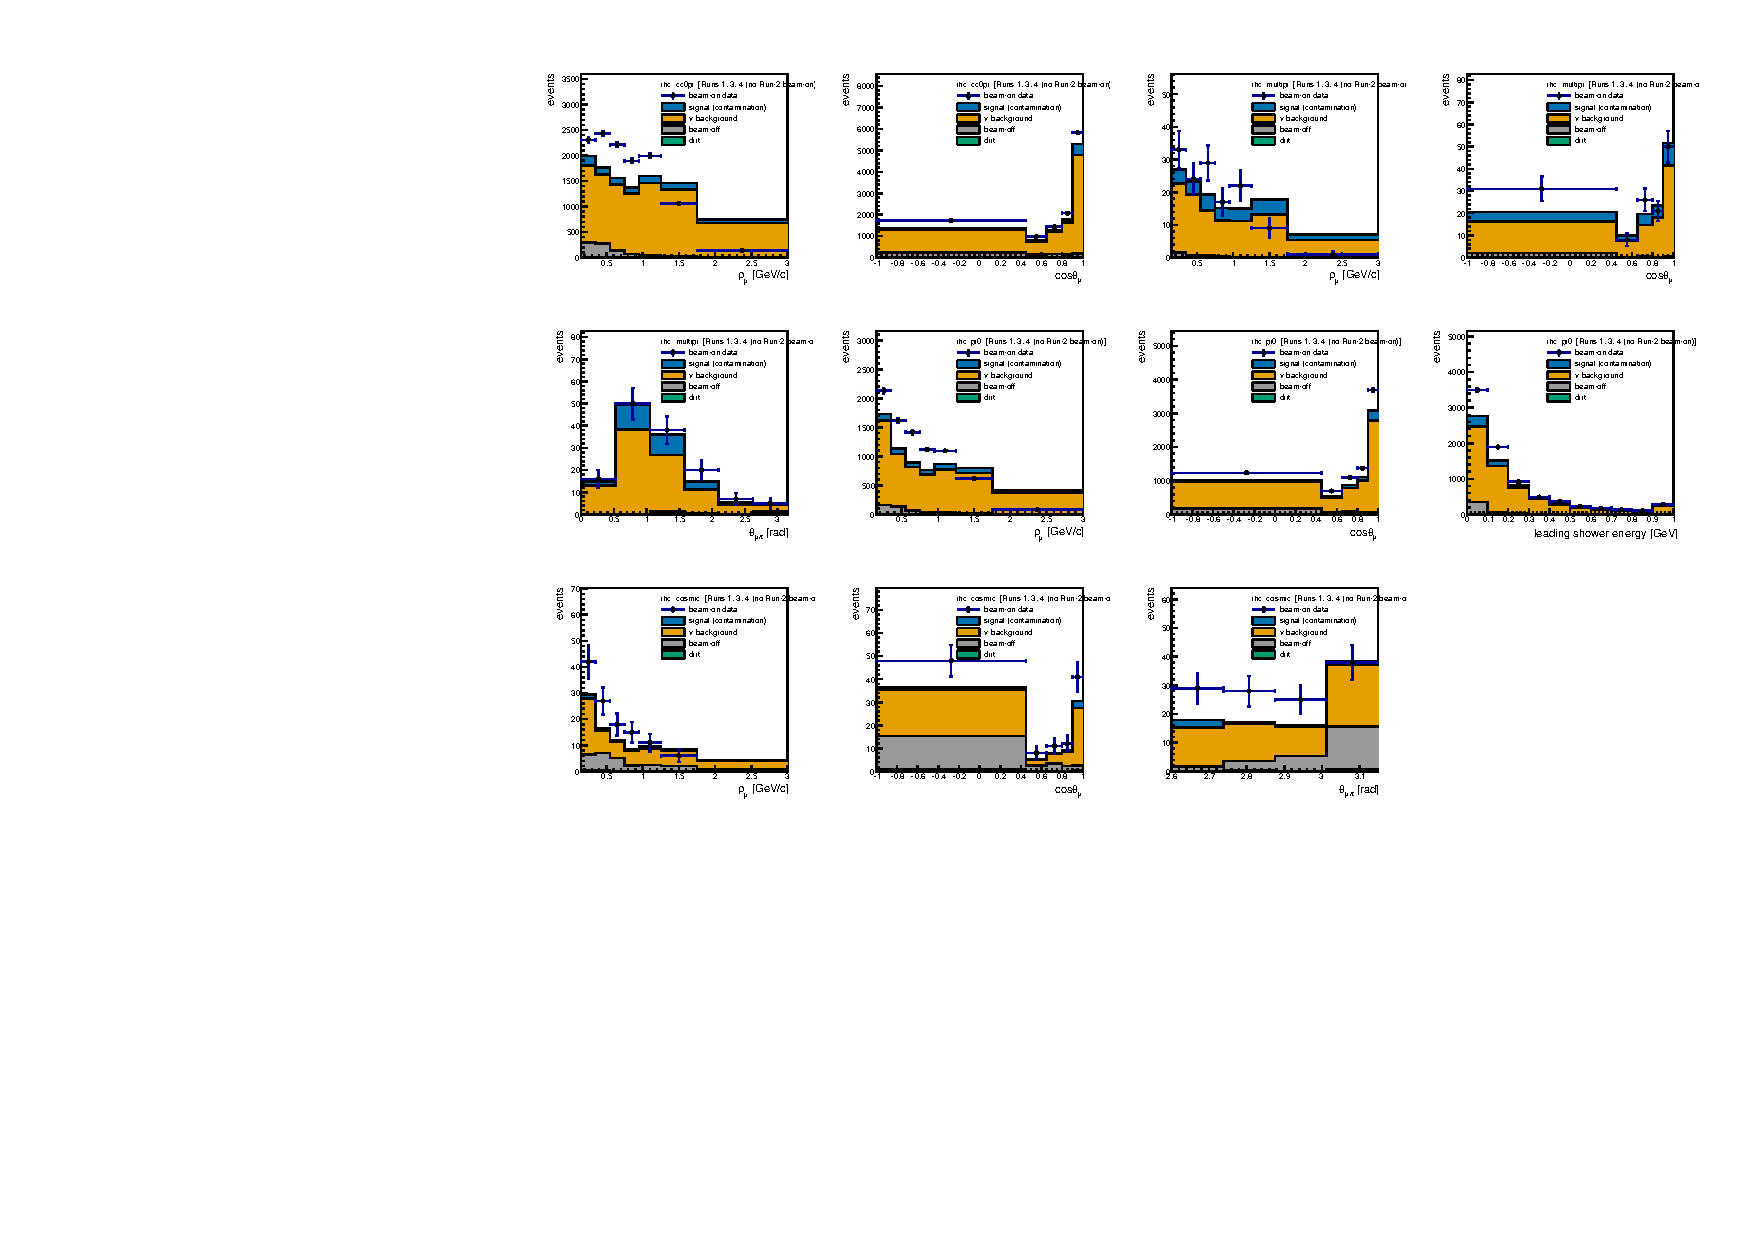
\includegraphics[width=\textwidth]{sideband_data_rhc}
  \caption{RHC control regions with beam-on data (Runs 1, 3, 4). Same layout as
    Fig.~\ref{fig:data_fhc}.}
  \label{fig:data_rhc}
\end{figure}

% =============================================================================
\section{The run-by-run comparison}
\label{sec:perrun}
% =============================================================================

The frozen procedure asks for the comparison run period by run period, and it is what
makes the mode-level numbers of \S\ref{sec:yields} uninterpretable as they stand.

\begin{table}[H]
  \centering
  \caption{Data over prediction, per run period and region. Each period's prediction uses
    that period's Monte Carlo scaled to its own exposure, its own beam-off sample and gate
    ratio, and the dirt scaled to its exposure. FHC Run~1 is the outlier; every other
    period of either mode lies between $0.83$ and $1.51$, with the high-statistics regions
    between $1.08$ and $1.25$.}
  \label{tab:perrun}
  \small
  \begin{tabular}{lcrrrr}
    \toprule
    Period & POT ($10^{20}$) & CC$0\pi$ & multi-$\pi$ & $\pi^0$ & cosmic \\
    \midrule
    FHC Run 1 & 3.283 & \textbf{0.637} & 0.911 & \textbf{0.715} & \textbf{0.595} \\
    FHC Run 4 & 2.075 & 1.173 & 1.217 & 1.248 & 1.141 \\
    FHC Run 5 & 2.231 & 1.135 & 0.899 & 1.188 & 1.200 \\
    \midrule
    RHC Run 1 & 0.605 & 1.191 & 1.076 & 1.086 & 0.828 \\
    RHC Run 3 & 5.003 & 1.150 & 1.243 & 1.246 & 1.510 \\
    RHC Run 4 & 2.883 & 1.115 & 0.823 & 1.201 & 1.248 \\
    \bottomrule
  \end{tabular}
\end{table}

\paragraph{FHC Run 1 is not a systematic of the prediction.}
The flux uncertainty is a hadron-production model uncertainty common to every run period
of a beam mode, and the detector variations are taken from the same Run-4 samples for all
periods, so both are almost fully correlated between run periods and cancel in a
period-to-period comparison. A prediction systematic can move all FHC periods together;
it cannot put Run~1 at $0.64$ while Runs~4 and~5 sit at $1.17$ and $1.14$. The effect is
also flat across the four regions of Run~1 --- $0.64$, $0.91$, $0.72$, $0.60$ --- which is
the signature of a normalisation applied to the whole period rather than of a
mis-modelled background class, since the four regions have very different compositions.

The quantity that is not verified anywhere in this comparison is the Run-1 FHC beam-on
exposure itself. The prediction is scaled to $3.283\times10^{20}$~POT and the beam-off to
$9\,846\,635$ beam-on gates, both taken from the trigger table; the beam-on ntuples carry
no exposure record of their own, so nothing here cross-checks them against the file that
was actually staged. The staged FHC Run-1 file spans runs 4952--6748 and the RHC Run-1
file begins at run 6748, so Run~1 is split between the horn modes inside the run range,
which is exactly the situation in which a partial file or a mis-assigned split is easy to
miss. The size of the effect is a concrete, falsifiable prediction. Every component of the
Run-1 prediction --- the Monte Carlo through its POT scale, the beam-off through its gate
ratio, the dirt through its exposure --- is proportional to the assumed Run-1 exposure, so
an exposure error rescales the whole prediction. Bringing FHC Run~1 onto the
$1.15$--$1.20$ of the other periods requires the true exposure to be a fraction
$f\simeq0.51$--$0.62$ of the assumed one, that is roughly $1.7$--$2.0\times10^{20}$~POT
in place of $3.283\times10^{20}$, with the three high-statistics regions giving
$f=0.55$ (CC$0\pi$), $0.62$ ($\pi^0$) and $0.51$ (cosmic). The consistency of $f$ across
regions of different composition is itself the evidence that a single multiplicative
exposure factor, and not a background class, is what is wrong. If instead the trigger
table is confirmed against the staged file, the deficit is real and must be treated as a
localised reconstruction failure under the response tree.

\paragraph{The remaining five periods carry a common offset.}
Setting FHC Run~1 aside, the five other periods sit above the prediction by $10$--$25\%$
in the high-statistics regions, in both beam modes. This is a common normalisation
offset. It is within the $20$--$30\%$ prediction uncertainty, and it is the one direction
the global test of \S\ref{sec:protocol} is built to be insensitive to, because the
correlated flux, cross-section and detector terms absorb it. Two features are worth
recording for whatever investigation follows: the offset appears in regions whose
beam-off fraction ranges from $3$--$5\%$ (multi-$\pi$) to $28$--$39\%$ (cosmic), which
argues against a beam-off scaling error; and it appears in both horn modes, which argues against a
mode-specific flux problem.

% =============================================================================
\section{The frozen comparison procedure applied to the data}
\label{sec:protocol}
% =============================================================================

\emph{[Protocol statistics being computed; this section is filled from the run in progress.]}

% =============================================================================
\section{What this establishes, and what it does not}
\label{sec:conclusions}
% =============================================================================

\begin{itemize}\itemsep3pt
  \item The processing chain runs on real beam-on data of both productions, pre-CRT and
    CRT-era, without error, and the blinding mechanism behaves as designed: no
    signal-region event was written, and the outputs are refused by the extraction.
  \item The control-region distributions are complete and are shown for the first time
    against data.
  \item \textbf{No conclusion about the background model should be drawn yet.} Two
    bookkeeping issues sit in front of any such conclusion: the missing Run-2 exposure,
    which is excluded consistently here but leaves $19\%$ of the analysis unexamined, and
    the FHC Run-1 anomaly, which has the size and the flatness of an exposure error.
  \item The frozen procedure's own response tree treats a single-period excursion as a
    reconstruction or exposure issue to be investigated, not as a model correction, and
    forbids excluding a period without independent evidence of a defect. That is the path
    FHC Run~1 should follow.
\end{itemize}

\paragraph{Required next.}
\begin{enumerate}[itemsep=3pt]
  \item Confirm the exposure and gate count of the staged FHC Run-1 beam-on file against
    the trigger table, and confirm that the FHC/RHC split of Run~1 at run 6748 is the one
    the exposure table assumes.
  \item Establish whether Run-2 beam-on data exist upstream. If they do, stage and process
    them; if they do not, Run~2 must be removed from the exposure and the whole
    normalisation regenerated.
  \item Repeat this comparison once both are settled, and only then read the
    normalisation offset of \S\ref{sec:perrun} as a statement about the background.
  \item The prerequisites for opening the signal region are unchanged and none of them is
    met by this note: the alternative-generator closure, the flux central-value
    confirmation, the MCS momentum bound, the clean-cache reproduction, and the
    inverted-PID regions for the misidentification transfers.
\end{enumerate}

\paragraph{Provenance.}
Beam-on skim written 2026-09-09 from the eight files of Table~\ref{tab:files}; prediction
from the release of 2026-09-06 (the same Monte Carlo, beam-off and dirt samples, and the
same per-run exposure scaling, as the blind studies), with Run~2 removed from both sides.

\end{document}
